\documentclass[a4paper, 12pt]{article}
\usepackage{graphicx}
\usepackage[a4paper, top=2cm , bottom=2cm , right=2cm , left=2cm ]{geometry}
\usepackage{graphicx} % Required for inserting images
\usepackage[T1]{fontenc}
\usepackage[latin1]{inputenc}
\usepackage{glossaries}
\usepackage{graphicx}
\usepackage{amsfonts}
\usepackage[hidelinks]{hyperref}
\usepackage{pifont}
\usepackage{eufrak}
\usepackage{float}
\usepackage{verbatim}
\usepackage{amssymb}
\usepackage{listings}
\usepackage{amsthm}
\usepackage{matlab-prettifier}
\usepackage{pifont}
\usepackage{multicol}
\usepackage{verbatim}
\usepackage{tikz}
\usetikzlibrary{shapes,arrows}
\usepackage{tikz}
\tikzstyle{mybox} = [draw=black, thin, rectangle, rounded corners, inner ysep=5pt, inner xsep=5pt, fill=blue!15]
\newtheorem{theorem}{Theorem}

\usepackage[affil-it]{authblk}

\title{\textbf{$\mathcal{H}_\infty$ synthesis: Weighting functions design }}

\author{Carlo Migliaccio
%\\Master's Degree in Computer Engineering\\
%Politecnico di Torino}
}
\date{November 2024}
\begin{document}
    \maketitle

    \section{Introduction}
    In the framework of $\mathcal{H}_\infty$ optimization for designing a control system, \textbf{weighting functions} are used in order to approximate by using rational functions some constraints in the frequency domain on the sensitivity function $S(s)$ and the complementary sensitivity function $T(s)$. Such constraints are derived by suitably traducing given specifications for the feedback control system. Roughly speaking at the end of the design (if we want to obtain robust stability and nominal performances) we want to impose: 
\begin{equation}
        \Bigg\Vert 
        \begin{aligned}
            W_1 S_n\\
            W_2 T_n
        \end{aligned}
        \Bigg\Vert_\infty < 1, \quad W_1=W_S, \quad 
        W_2=\max(W_T, W_U)
    \end{equation}
    Where $S_n$, $T_n$ are related to the \textit{nominal model}.

    \section{Weighting function $W_S^{-1}(s)$ ($\nu+p=1$)}
    We can explicit the constraints on the sensitivity function $S(s)$ using the following inequality: 
    \begin{equation}
        \Vert W_S(j\omega)S(j\omega) \Vert_\infty < 1
    \end{equation}
    This is the same to state the for all frequencies $\omega$, $S(s)$ must lie below $W_S^{-1}(s)$. This weighting function is in general the most complicate to design since, when the requirements are translated, different types of constraints comes up:
    \vspace{-0.2cm}
    \begin{enumerate}
        \itemsep-0.3em
        \item A constraint on the shape of $s^{\nu+p}S^*{(0)}$ for $\omega\to0$
        \item A constraint on the level of attenuation for \textit{low frequencies}, what we call $M_S^{LF}$; 
        \item A constraint in the \textit{high frequency} range due to the peak of $S(s)$ of a prototype second order system; 
    \end{enumerate}
    Clearly, it could be that some of this constraints are not present for example the attenuation $M_S^{LF}$ due to a sinusoidal disturbance $d_p(t)$ on the output of the plant.
    Beyond this constraints, it is useful at this stage to keep in mind the shape of the prototype second order system $S^{II}(s)$:
    \begin{equation}
        S^{II}(s)=\frac{s(\frac{s}{\omega_n^2}+\frac{2\zeta}{\omega_n})}{(1+\frac{2\zeta}{\omega_n}s+\frac{s^2}{\omega_n^2})}
    \end{equation}
    It is remarkable that the transient requirements are mapped directly on such a type of prototype, then in the mid-range frequencies could be effective tempting to assume that shape. \\
    The introduction we have just done holds in general, then there are some critical aspects related to the design of the weighting function which is related to the system type $\nu+p$. 
    In the following we show some significant examples for weighting functions embedding the constraints on $S(s)$.

    \subsection{Second order polynomials}
    Here we want to imitate the shape of $S^{II}(s)$ only in the neighborhood of $\omega_n$. An example of such a type of weighting function is reported in Figure (\ref{fig: type1_2nd}). 
    \begin{figure}[h]\label{fig: type1_2nd}
        \centering
        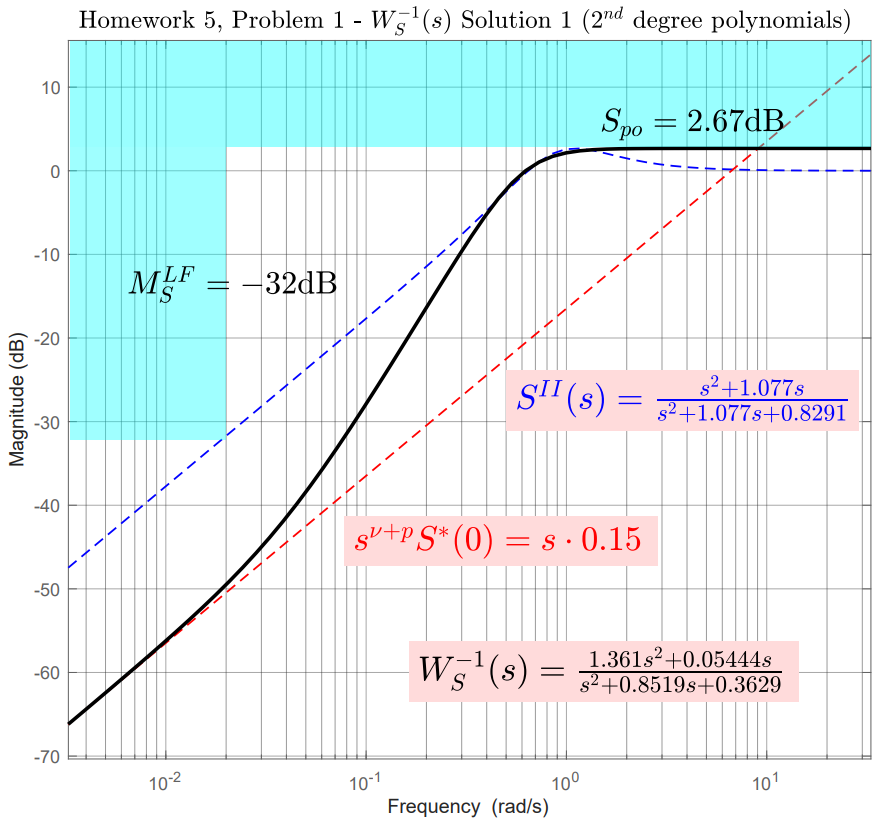
\includegraphics[scale=0.8]{img/Ws_type1_second.png}
        \caption{$W_S^{-1}(s)$, system-type 1, second order polynomials}
    \end{figure}
    The general form for such a type of function is: 
    {\large{
        \begin{equation}
            W_S^{-1}(s) = a{s^{1}} \frac{1+\frac{s}{\omega_1}}{{(1+\frac{2\zeta}{\omega_2}s+\frac{s^2}{\omega_2^2})}}
        \end{equation}
    }}
    About the parameters: 
    \begin{itemize}
        \itemsep-0.3em
        \item The gain $a$ is chosen by computing 
        \begin{equation}
            \lim_{s\to{0}} \frac{1}{s}W_S^{-1}(s)=S^{*}(0)
        \end{equation}
        in this way for $s\to0$ the function will be exactly the red dashed line; 
        \item for the zero at $\omega_1$ there is not a precise choice if $M_S^{LF}$ is present a frequency around $\omega_p$ can be chosen, otherwise by a trial and error procedure you can chose a frequency such that at a certain point $W_S$ could reach $S^{II}(s)$; 
        \item In order to imitate the shape of $S^{II}(s)$ around $\omega_n$ a pair of complex conjugate poles are used. The frequency $\omega_2$ can be chosen by solving the following equation:
        \begin{equation}\label{eq:Spo_limit}
            S_{po}=\lim_{s\to{\infty}} W_S^{-1}(s)
        \end{equation}
        \noindent
        The damping factor initially could be $\zeta=0.707$ in order to use a \textit{Butterworth polynomial}, but it is only a guideline, you can increase/decrease this value so that the functions in the range of the "bump" could be as similar  as possible.
    \end{itemize}

    \subsection{Third order polynomials}
 
    In order to obtain better results from the optimizer solving the $\mathcal{H}_\infty$ optimization, higher order polynomial can be used in order to better approximate the behaviour of the prototype second order system. As we have done before, an example of this is reported in Figure (\ref{fig:type1_3rd})

    \begin{figure}\label{fig:type1_3rd}
        \centering
        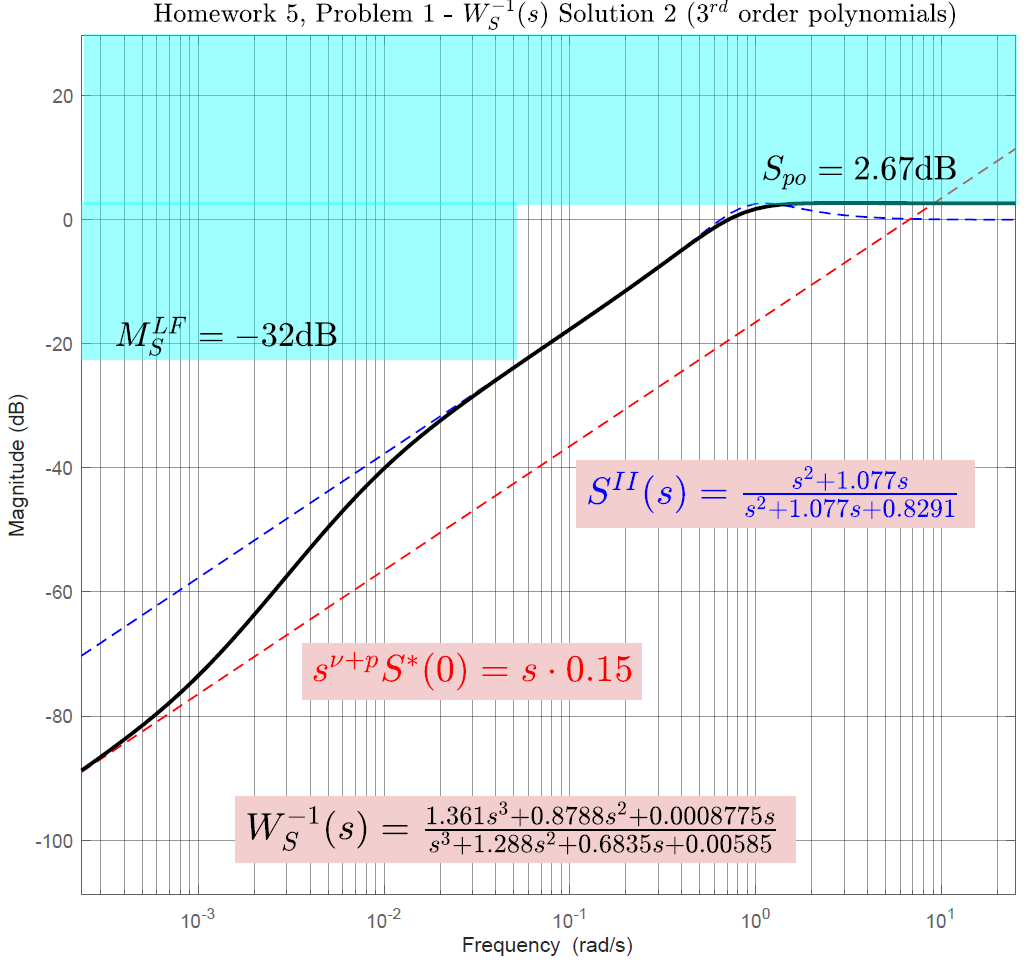
\includegraphics[scale=0.7]{img/Ws_type1_third.png}
        \caption{$W_S^{-1}(s)$, system-type 1, third order polynomial}
    \end{figure}
    The shape of such a function is the following:
    {\large{
        \begin{equation}
            W_S^{-1}(s) = a{s^{1}} \frac{
                \bigl(1+\frac{s}{z_1}\bigr)
                \bigl(1+\frac{s}{z_2}\bigr)
            }
            {
                {(1+\frac{2\zeta}{\omega}s+\frac{s^2}{\omega^2})}
                {\bigl(1+\frac{s}{p}\bigr)}
            }
        \end{equation}
    }}
    Here a pair zero-pole ($z1$, $p$) is used in order to reach the prototype second order sooner as possible, a pair of complex conjugate poles is used to model $W_S^{-1}$ around $\omega_n$, an $\omega$ similar to $\omega_n$ could be a good choice. The pole $p$ is chosen as in (\ref{eq:Spo_limit}) in order to reach the peak $S_{po}$ in the \textit{high-frequency range}. 

    \section{Weighting function $W_S^{-1}(s)$ ($\nu+p=2$)}
    Whether from the requirement translation comes up that $\nu+p=2$, then the red dashed line and $S^{II}$ at LF\footnote{
        From now on LF $\to$ Low Frequency
    } are not parallel anymore. 

    \begin{figure}[h]\label{fig: type2_2}
        \centering
        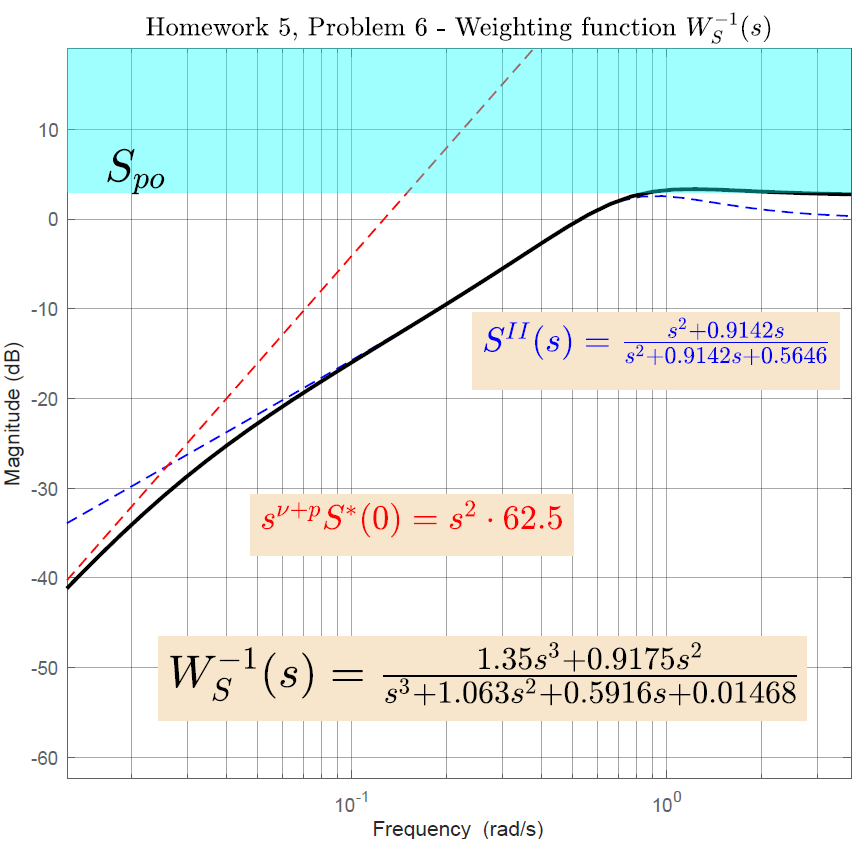
\includegraphics[scale=0.8]{img/Ws_type2_2.png}
        \caption{$W_S^{-1}(s)$, system-type 2}
    \end{figure}

    \noindent
    The shape for $W_S^{-1}(s)$ in this case is:
    {\large{
        \begin{equation}
            W_S^{-1}(s) = a{s^{2}} \frac{
                \bigl(1+\frac{s}{z}\bigr)
            }
            {
                {(1+\frac{2\zeta}{\omega}s+\frac{s^2}{\omega^2})}
                {\bigl(1+\frac{s}{p}\bigr)}
            }
        \end{equation}
    }}
    The parameter $a$ is chosen according to the same principle as before. Moreover, around the intersection point between $s^2{S^*(0)}$ we place a pole at the frequency $p$, then a complex conjugate pair is added in order to model the 'bump' around $\omega_n$, in order to obtain a slope of 0 dB/dec a zero at the frequency $z$ is needed. The zero is chosen imposing that the condition (\ref{eq:Spo_limit}) is met.
    
    \begin{comment}
    \section{Weighting function $W_S^{-1}(s)$ ($\nu+p=0$)}
    When we have $\nu+p=0$ for $\omega\to{0}$ our function is constant; in order to gain until a certain point 20 dB/dec, we insert a zero, then, as usual, the complex-conjugate pair. Finally in order to control the behaviour at HF, a zero in $z_2$ is added (as usual compute the limit to infinity). The shape in this case is:
    {\large{
        \begin{equation}
            W_S^{-1}(s) = a{s^{0}} \frac{
                \bigl(1+\frac{s}{z_1}\bigr)
                \bigl(1+\frac{s}{z_2}\bigr)
            }
            {
                {(1+\frac{2\zeta}{\omega}s+\frac{s^2}{\omega^2})}
            }
        \end{equation}
    }}
    %WS=(a*(1+s/z1)*(1+s/z2))/(1+(2*0.7/w1)*s+(s/w1)^2)

    \begin{figure}[h]
        \centering
        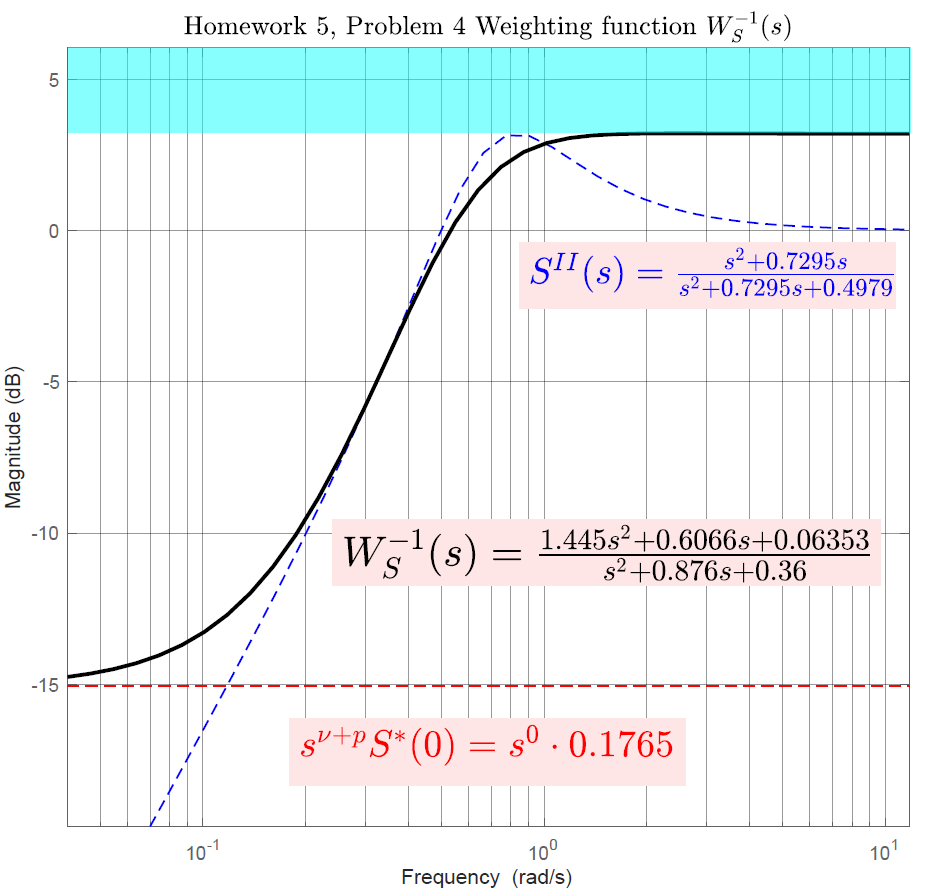
\includegraphics[scale=0.7]{img/Ws_type0.png}
        \caption{$W_S^{-1}(s)$, system-type 0}
    \end{figure}
    \end{comment}
    

    \section{Weighting function $W_T(s)$}
    Good news: the design of the weighting function on $T(s)$ is simpler. We recall that in the phase of requirements translation we derive (at most) two constraints: (i) the first due to the sinusoidal disturbance at HF on the sensor, (ii) the second related to the maximum resonance peak $T_po$ derived from the requirement on the overshoot $\hat{s}$. The shape of such a rational function is always the same: 
    \begin{equation}
        W_T^{-1}(s) = \frac{T_{po}}{{(1+\frac{2\zeta}{\omega_T}s+\frac{s^2}{\omega_T^2})}}
    \end{equation}
    The parameter $\omega_T$ is chosen by trial and error so that the $W_T^{-1}(s)$ could perfectly pass for the corner imposed by the pair ($\omega_s$, $M_T^{HF}$). 
    An example is reported in the following figure.

    \begin{figure}[h]
        \centering
        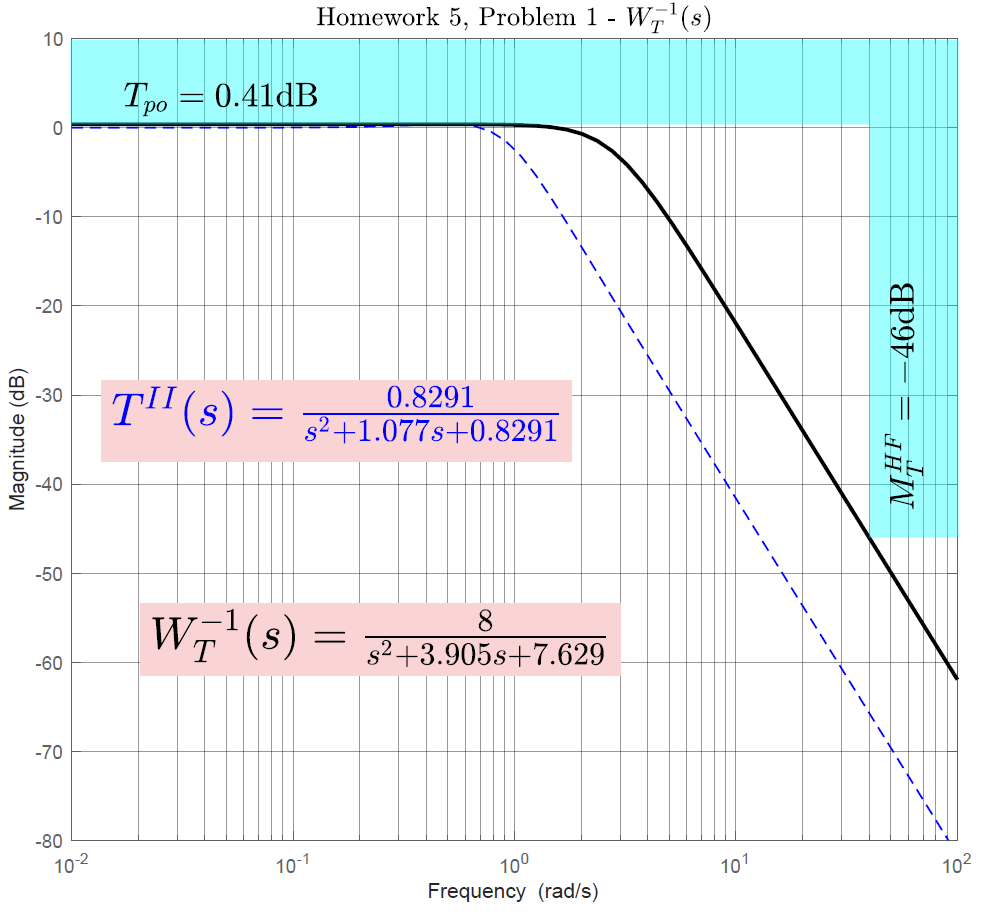
\includegraphics[scale=0.7]{img/Wt.png}
        \caption{Weighting function $W_T^{-1}(s)$ on $T(s)$}
    \end{figure}
    
    \section{Weighting function $W_U(s)$}
    Despite our best effort to approximate real dynamical systems, there is always uncertainty which could be either dynamical (this is due to the neglection of some parts of the system), or \textit{parametric} (this  is due to the uncertainty on the parameters entering in the mathematical description of a certain system for example by using a transfer function). Different approaches for describing the uncertainty can be considered.

    \subsection{Additive uncertainty model}
    In this case the \textbf{real plant} is considered as a member of a family of systems which can be described by the set 
    \begin{equation}\label{eq:Ma}
        M_a = \{
            G_p(s)=G_{pn}(s)+W_U(s)\Delta(s), \quad \Vert \Delta(s) \Vert_\infty \le 1 
        \}
    \end{equation}
    where $G_p(s)$ is a member of the family, $G_{pn}(s)$ is a given \textbf{nominal plant}, $W_U(s)$ is a \textbf{weighting function} taking into account (frequency-by-frequency) the maximum uncertainty entering into the problem, finally $\Delta(s)$ is any transfer function whose $\mathcal{H}_\infty$ norm is less than one.\\
    If we go deeper and retrieve the expression of $\Delta(s)$ we can write that
    \begin{equation}\label{eq:cloud_a}
        \vert G_p(j\omega)-G_{pn}(j\omega)    \vert \le \vert W_U(j\omega) \vert \quad \forall \omega \iff
        \vert W_U(j\omega) \vert   \ge  \vert G_p(j\omega)-G_{pn}(j\omega)    \vert
    \end{equation}
    This gives us useful information on the weighting function $W_U(s)$ that must lie above the \textit{transfer functions cloud} obtained by gridding the parameter space and drawing the function $\vert G_p(j\omega)-G_{pn}(j\omega) \vert$ for each combination of the parameters entering into the description of the \textbf{real uncertain plant}. (see Homework 6, \textsf{Problem A}).
    By using the (\ref{eq:Ma}) we can represent such a model of uncertainty by using the following block diagram:

    \begin{figure}
        \centering
        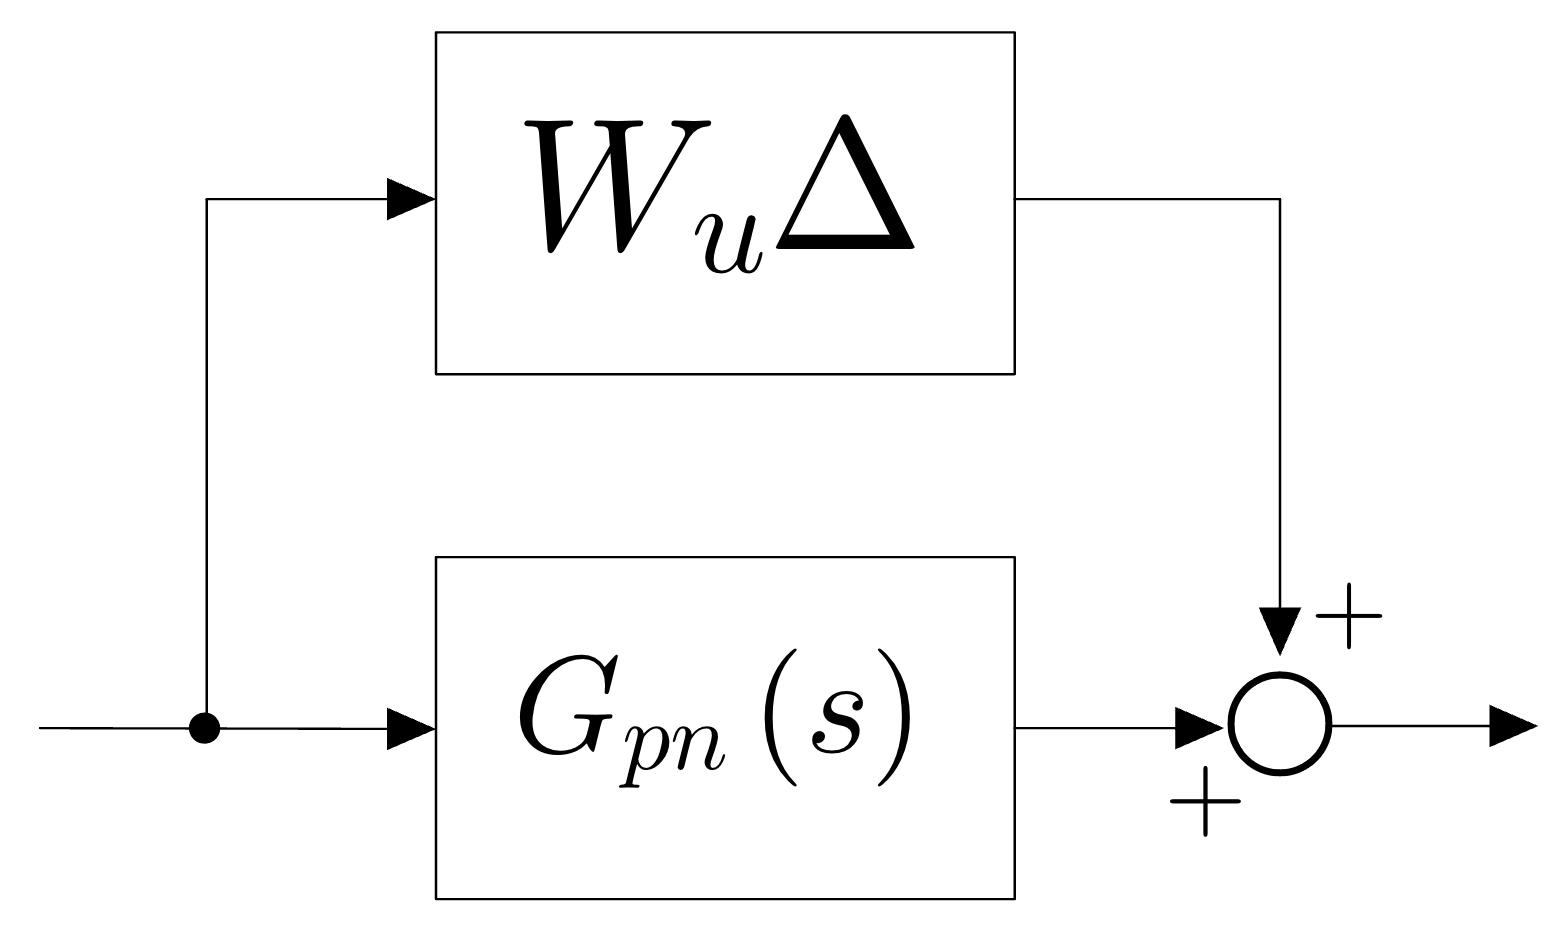
\includegraphics[scale=0.2]{img/Additive.jpeg}
        \caption{Additive uncertainty model (Block diagram)}
    \end{figure}


    \subsection{Multiplicative uncertainty model}
    Here the real uncertain plant is considered as part of a set of a dynamical system $M_m$ described by: 
    \begin{equation}
        M_m = \{
            G_p(s) = G_{pn}(s) (1 + W_U(s) \Delta(s)), \quad 
            \Vert \Delta(s) \Vert \le 1
        \}
    \end{equation}
    Where $G_p(s), \ G_{pn}(s), \ \Delta(s), W_U(s)$ are defined as before. What is different in this case is the relationship between $\Delta(s)$ and the weighting function $W_U(s)$. By doing simple calculation and applying the definition of $\mathcal{H}_\infty$ norm\footnote{
        The $\mathcal{H}_\infty$ norm is defined as:
        \begin{equation*}
            \Vert H(s) \Vert_\infty 
        = \max_{\omega} \vert H(j\omega) \vert
        \end{equation*}
        where $H: \mathbb{C} \to \mathbb{C}$ is a complex function of the complex variable $s$.
    } we obtain:
    \begin{equation} \label{eq:cloud_m}
        \vert W_U(j\omega) \vert \ge
        \bigg\vert
            \frac{G_p(j\omega)}{G_{pn}(j\omega)}-1
        \bigg\vert \quad \forall \omega
    \end{equation}
    
    \begin{figure}[h]
        \centering
        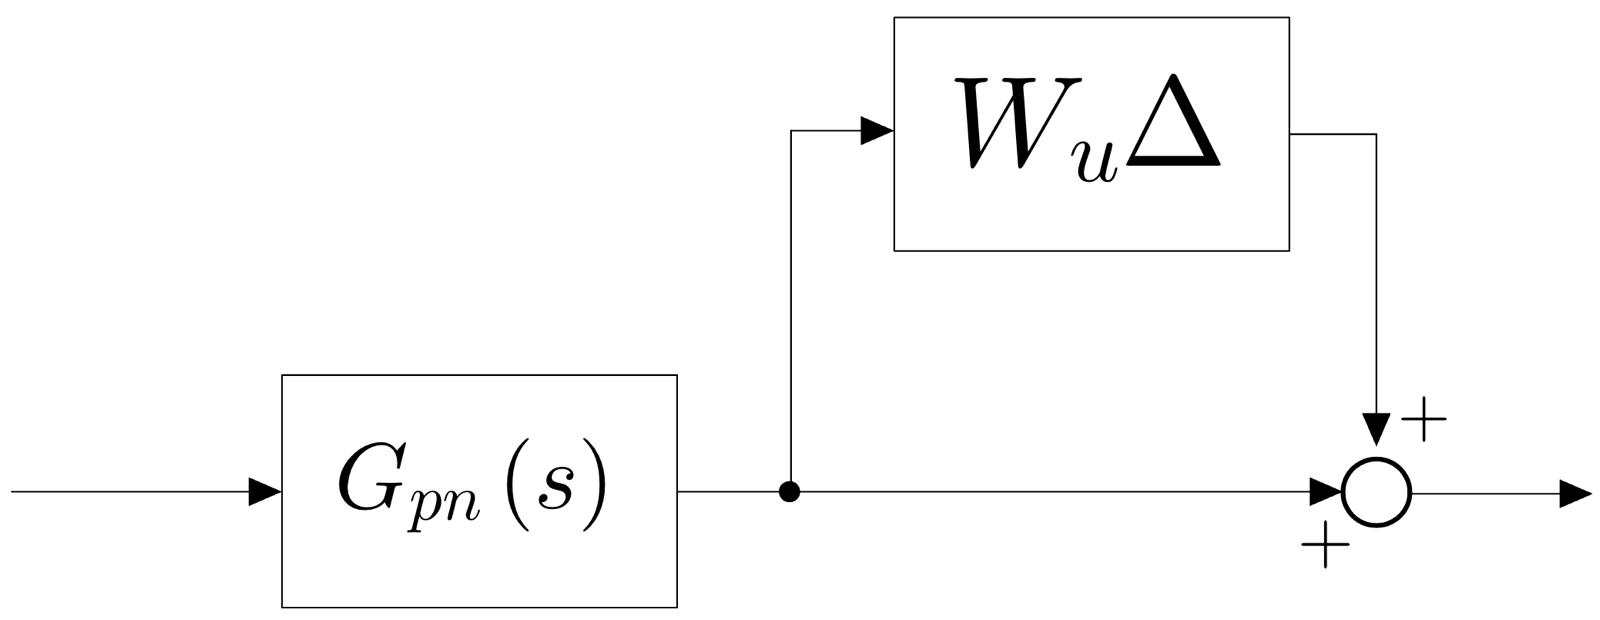
\includegraphics[scale=0.2]{img/Multiplicative.jpeg}
        \caption{Multiplicative Uncertainty Interval (block diagram)}
    \end{figure}


    \subsection{Obtaining a nominal plant given the PUI}
    Before going on the description of the method by which a $W_U(s)$ is obtained, we have to deal with an issue which is directed linked to our problems: given a plant described by a transfer function in which some parameters enters and are described by the Parameter Uncertainty Intervals (PUI), \textbf{how can we obtain a nominal model for the plant under analysis?} \\
    The statistics says us that peeking the average of the extrema for each parameter we obtain the minimum uncertainty. That is \textit{the center of each PUI guarantees the minimum uncertainty}. This is not always true, but for the cases of our interest is a good technique in order to retrieve the nominal model. Let us give an example:
    \begin{equation}
        G_p(s) = K \frac{(1+\frac{1}{z_1})}{(1+\frac{1}{p_1})}, \ 
        K \in [\underline{K}, \overline{K}], \
        z_1 \in [\underline{z}_1, \overline{z}_1]\
        p_1 \in [\underline{p}_1, \overline{p}_1]
    \end{equation}
    The nominal model is:
    \begin{equation}
        G_{pn}(s) = K_n \frac{(1+\frac{1}{z_{1n}})}{(1+\frac{1}{p_{1n}})}, \quad
        K_n = \frac{\underline{K}+ \overline{K}}{2} \ 
        z_{1n} = \frac{\underline{z}_1+ \overline{z}_1}{2} \ 
        p_{1n} = \frac{\underline{p}_1+\overline{p}_1}{2} \ 
    \end{equation}
    Note that this is the unstructured way to describe structured uncertainty, other techniques provide us with the possibility to dealing with structured uncertainty without conservativeness ($\mu$-analysis).

    \subsection{On the design of $W_U(s)$}
    From the previous paragraphs we have understood that the weighting function $W_U(s)$ must lie above the cloud generated by (\ref{eq:cloud_a}) or (\ref{eq:cloud_m}). There are mainly two ways to design it:
    \begin{enumerate}
        \itemsep-0.3em
        \item \textbf{By Hand}, in the sense that a transfer function $W_U(s)$ is implemente by adding zeros and poles and considering the following constraints:
        \begin{align}
            &\lim_{s\to{0}} W_U(s)=W_U^{0}\\
            &\lim_{s\to{\infty}} W_U(s)=W_U^{\infty}  
        \end{align}
        where $W_U^0$ and $W_U^\infty$ can be found empirically by analyzing the graph.
        \item \textbf{By using the \texttt{fitmag} command}, in this case a proper choise is to pick frequency-by-frequency the maximum gain of the function $\Delta_a(s)$ or $\Delta_m(s)$ (additive or multiplicative).
    \end{enumerate}
    In the following the family of transfer functions and the weight $W_U(s)$ is showed in the case the second method is used.

    \begin{figure}[h]
        \centering
        \includegraphics[scale=0.7]{img/Wu.eps}
        \caption{Transfer functions cloud and $W_U(s)$}
    \end{figure}


 
\end{document}
